% Options for packages loaded elsewhere
\PassOptionsToPackage{unicode}{hyperref}
\PassOptionsToPackage{hyphens}{url}
\documentclass[
  11pt,
  fontset=fandol]{ctexart}
\usepackage{xcolor}
\usepackage[a4paper,margin=22mm]{geometry}
\usepackage{amsmath,amssymb}
\setcounter{secnumdepth}{-\maxdimen} % remove section numbering
\usepackage{iftex}
\ifPDFTeX
  \usepackage[T1]{fontenc}
  \usepackage[utf8]{inputenc}
  \usepackage{textcomp} % provide euro and other symbols
\else % if luatex or xetex
  \usepackage{unicode-math} % this also loads fontspec
  \defaultfontfeatures{Scale=MatchLowercase}
  \defaultfontfeatures[\rmfamily]{Ligatures=TeX,Scale=1}
\fi
\usepackage{lmodern}
\ifPDFTeX\else
  % xetex/luatex font selection
\fi
% Use upquote if available, for straight quotes in verbatim environments
\IfFileExists{upquote.sty}{\usepackage{upquote}}{}
\IfFileExists{microtype.sty}{% use microtype if available
  \usepackage[]{microtype}
  \UseMicrotypeSet[protrusion]{basicmath} % disable protrusion for tt fonts
}{}
\makeatletter
\@ifundefined{KOMAClassName}{% if non-KOMA class
  \IfFileExists{parskip.sty}{%
    \usepackage{parskip}
  }{% else
    \setlength{\parindent}{0pt}
    \setlength{\parskip}{6pt plus 2pt minus 1pt}}
}{% if KOMA class
  \KOMAoptions{parskip=half}}
\makeatother
\usepackage{longtable,booktabs,array}
\newcounter{none} % for unnumbered tables
\usepackage{calc} % for calculating minipage widths
% Correct order of tables after \paragraph or \subparagraph
\usepackage{etoolbox}
\makeatletter
\patchcmd\longtable{\par}{\if@noskipsec\mbox{}\fi\par}{}{}
\makeatother
% Allow footnotes in longtable head/foot
\IfFileExists{footnotehyper.sty}{\usepackage{footnotehyper}}{\usepackage{footnote}}
\makesavenoteenv{longtable}
\setlength{\emergencystretch}{3em} % prevent overfull lines
\providecommand{\tightlist}{%
  \setlength{\itemsep}{0pt}\setlength{\parskip}{0pt}}
\usepackage{float,caption,tikz,pgfplots}
\usepgfplotslibrary{groupplots}
\pgfplotsset{compat=1.18}
\setlength{\parskip}{.45em}
\setlength{\parindent}{0pt}
\setlength{\emergencystretch}{3em}
\pagestyle{plain}
\usepackage{bookmark}
\IfFileExists{xurl.sty}{\usepackage{xurl}}{} % add URL line breaks if available
\urlstyle{same}
\hypersetup{
  pdftitle={细胞核中心定位：从五轮实验看细胞核如何被找到------阶段报告8中文导读},
  pdfauthor={bdd26 research},
  hidelinks,
  pdfcreator={LaTeX via pandoc}}

\title{细胞核中心定位：从五轮实验看细胞核如何被找到------阶段报告8中文导读}
\author{bdd26 research}
\date{17 November 2026}

\begin{document}
\maketitle

{
\setcounter{tocdepth}{2}
\tableofcontents
\newpage
}
\subsection{这阶段要解决什么问题？}\label{ux8fd9ux9636ux6bb5ux8981ux89e3ux51b3ux4ec0ux4e48ux95eeux9898}

阶段报告 7 介绍到 P26。本报告接着讲 P27 至
P31：怎样训练病理图像模型，才能在显微图像中给更多细胞核找到中心？研究特别关注标注为凋亡或坏死的细胞核，以下简称死亡细胞核。

五轮使用同一批数据：2,134 张图像用于训练，另外 522
张用于开发评估。开发评估图像有 12,250 个标注细胞核，其中 145
个死亡细胞核的轮廓不接触图像边界。若一个预测点距标注中心不超过三像素，并在一对一配对中被分给该标注，就算找到这个细胞核。每轮都有同时训练的对照方案，两种方案各做两次独立训练，分别使用随机种子
19 和 1。随机种子控制训练中的随机过程。

\subsection{五轮实验分别改变了什么？}\label{ux4e94ux8f6eux5b9eux9a8cux5206ux522bux6539ux53d8ux4e86ux4ec0ux4e48}

模型的图像编码器有 24
层，可以理解为依次处理图像信息的一系列步骤。P27--P30 每次都只调整其中 12
层，但选取的位置不同；对照始终调整后 12 层。P31
保持对照的编码器训练位置，改变把图像特征转换为中心预测的检测头。

{\def\LTcaptype{none} % do not increment counter
\begin{longtable}[]{@{}
  >{\raggedright\arraybackslash}p{(\linewidth - 6\tabcolsep) * \real{0.2143}}
  >{\raggedright\arraybackslash}p{(\linewidth - 6\tabcolsep) * \real{0.2143}}
  >{\raggedleft\arraybackslash}p{(\linewidth - 6\tabcolsep) * \real{0.2857}}
  >{\raggedleft\arraybackslash}p{(\linewidth - 6\tabcolsep) * \real{0.2857}}@{}}
\toprule\noalign{}
\begin{minipage}[b]{\linewidth}\raggedright
轮次
\end{minipage} & \begin{minipage}[b]{\linewidth}\raggedright
改变的部分
\end{minipage} & \begin{minipage}[b]{\linewidth}\raggedleft
死亡细胞核匹配数变化（种子 19／1）
\end{minipage} & \begin{minipage}[b]{\linewidth}\raggedleft
全部细胞核的匹配变化
\end{minipage} \\
\midrule\noalign{}
\endhead
\bottomrule\noalign{}
\endlastfoot
P27 & 训练前 12 层 & +6／+15 & +521／+213 \\
P28 & 隔一层训练一层 & +2／−1 & +528／+273 \\
P29 & 训练前 6 层和后 6 层 & +16／+13 & +283／+165 \\
P30 & 训练中间 12 层 & +7／+15 & +648／+516 \\
P31 & 在检测头加入分组归一化 & +8／+2 & −140／+6 \\
\end{longtable}
}

每个数字都比较同轮、同一随机种子的两种方案。P29
在两次训练中都增加了较多死亡细胞核匹配；P30
在两次训练中找到了较多全部类别的细胞核，并减少了未匹配预测点。P31
分组归一化先按通道分组调整单张图像的特征，再学习缩放和偏移；它提高了训练图像上的检出率，两次开发评估的变化则不同。

\begin{figure}[H]\centering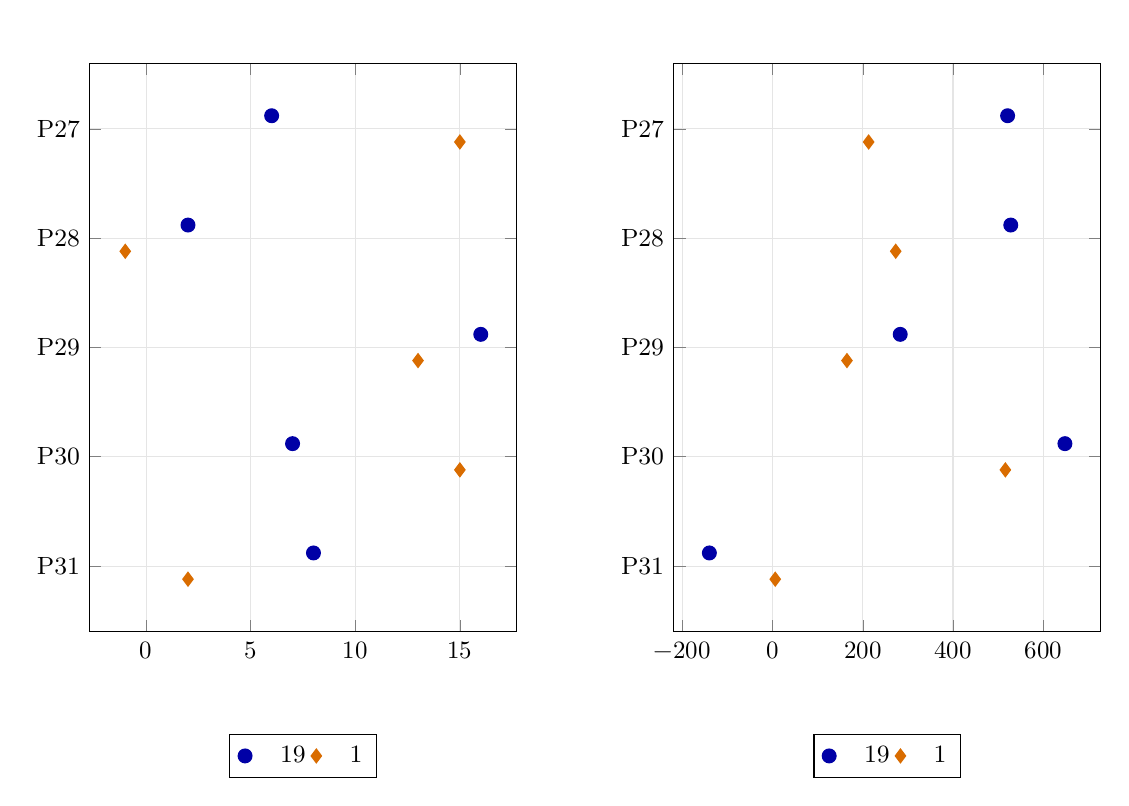
\begin{tikzpicture}
\begin{groupplot}[group style={group size=2 by 1,horizontal sep=2.0cm},width=7cm,height=8.8cm,ytick={0,1,2,3,4},yticklabels={P27,P28,P29,P30,P31},ymin=-.6,ymax=4.6,y dir=reverse,grid=major,grid style={gray!20},tick label style={font=\small},label style={font=\small},title style={font=\small},legend style={font=\small,at={(.5,-.18)},anchor=north,legend columns=2}]
\nextgroupplot[title={死亡细胞核匹配变化},xlabel={新方案减同轮对照：匹配数}]
\addplot[only marks,mark=*,mark size=2.5pt,color=blue!65!black] coordinates {(6,-0.12) (2,0.88) (16,1.88) (7,2.88) (8,3.88)};
\addlegendentry{种子 19}
\addplot[only marks,mark=diamond*,mark size=2.5pt,color=orange!85!black] coordinates {(15,0.12) (-1,1.12) (13,2.12) (15,3.12) (2,4.12)};
\addlegendentry{种子 1}
\nextgroupplot[title={全部细胞核匹配变化},xlabel={新方案减同轮对照：匹配数}]
\addplot[only marks,mark=*,mark size=2.5pt,color=blue!65!black] coordinates {(521,-0.12) (528,0.88) (283,1.88) (648,2.88) (-140,3.88)};
\addlegendentry{种子 19}
\addplot[only marks,mark=diamond*,mark size=2.5pt,color=orange!85!black] coordinates {(213,0.12) (273,1.12) (165,2.12) (516,3.12) (6,4.12)};
\addlegendentry{种子 1}
\end{groupplot}
\end{tikzpicture}
\caption{P27–P31 新方案相对同期对照的匹配数变化。左侧是死亡细胞核，右侧是全部细胞核；圆点和菱形分别表示种子 19 和 1。}\end{figure}

\subsection{看懂下面的组织图}\label{ux770bux61c2ux4e0bux9762ux7684ux7ec4ux7ec7ux56fe}

每组左右分别是同一张真实组织图像的对照结果与新方案结果。青色十字是预测的中心。白色圆圈表示两组都找到这个死亡细胞核；绿色表示只有新方案找到；橙色表示只有对照找到；粉色表示两组都漏掉。数字是标注对象编号，坐标按先行后列记录。两个随机种子使用相同的图像，但分别训练模型。

\subsection{P27：改训练前十二层，哪些核改变了？}\label{p27ux6539ux8badux7ec3ux524dux5341ux4e8cux5c42ux54eaux4e9bux6838ux6539ux53d8ux4e86}

\noindent

\begin{minipage}{\linewidth}\centering
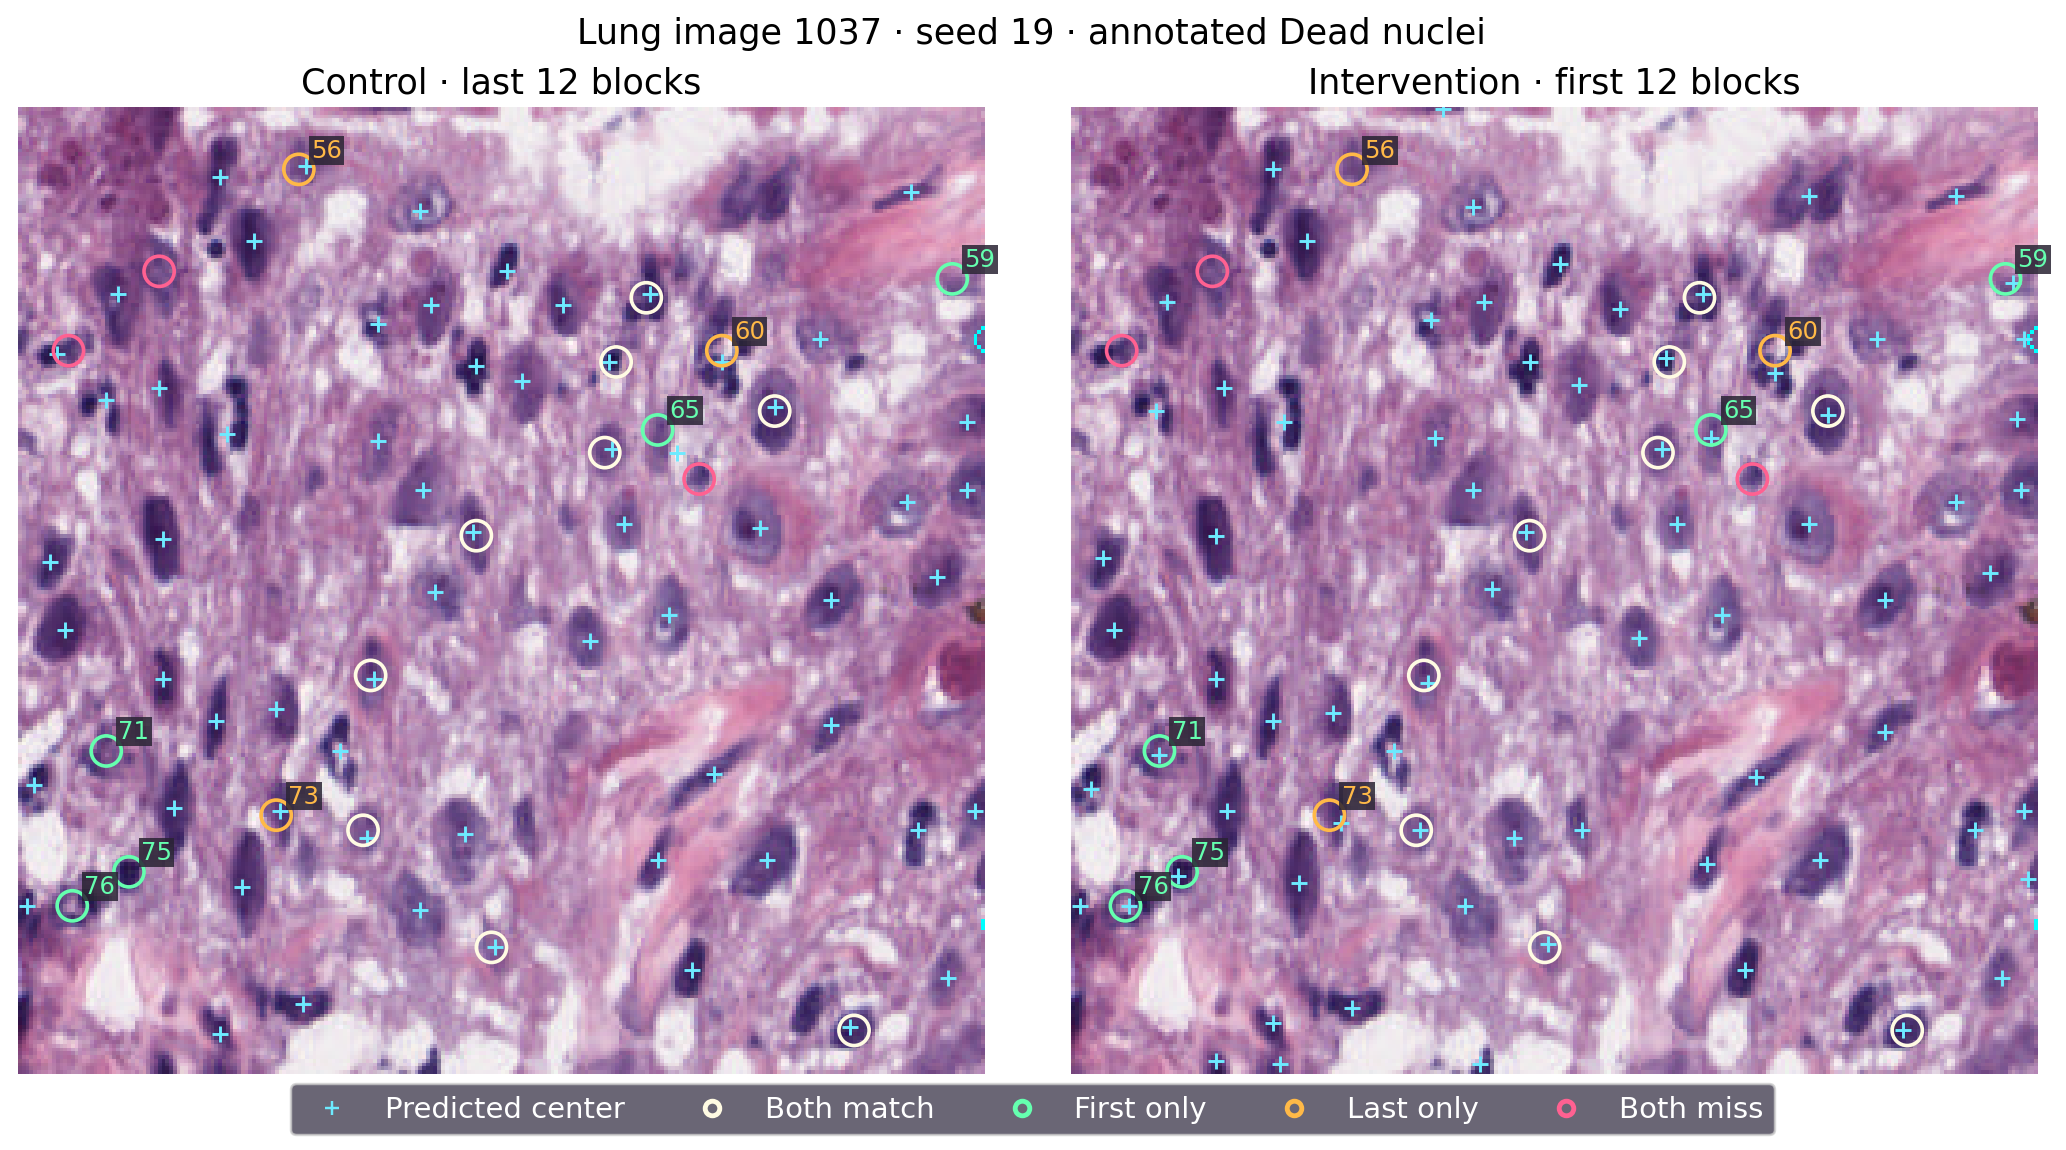
\includegraphics[width=\linewidth,height=.40\textheight,keepaspectratio]{assets/p27_image_1037_seed_19.png}
\captionof{figure}{P27 肺组织图像 1037，种子 19。左为训练后十二层的对照，右为训练前十二层的方案。圆圈颜色与预测十字符号见上文。}
\raggedright

该图从找到 20 个死亡细胞核中的 12 个，变为找到 14 个。对象 71 位于（170，23），对照中最近预测点相距 21.02 像素，新方案中缩短为 1 像素；对象 56 位于（16，74），最近预测距离从 2.24 增至 21 像素，丢失匹配。总数增加两个，实际上包含五个新增和三个丢失。

\end{minipage}

\subsection{P28：交错训练，为什么总数接近却对象不同？}\label{p28ux4ea4ux9519ux8badux7ec3ux4e3aux4ec0ux4e48ux603bux6570ux63a5ux8fd1ux5374ux5bf9ux8c61ux4e0dux540c}

\noindent

\begin{minipage}{\linewidth}\centering
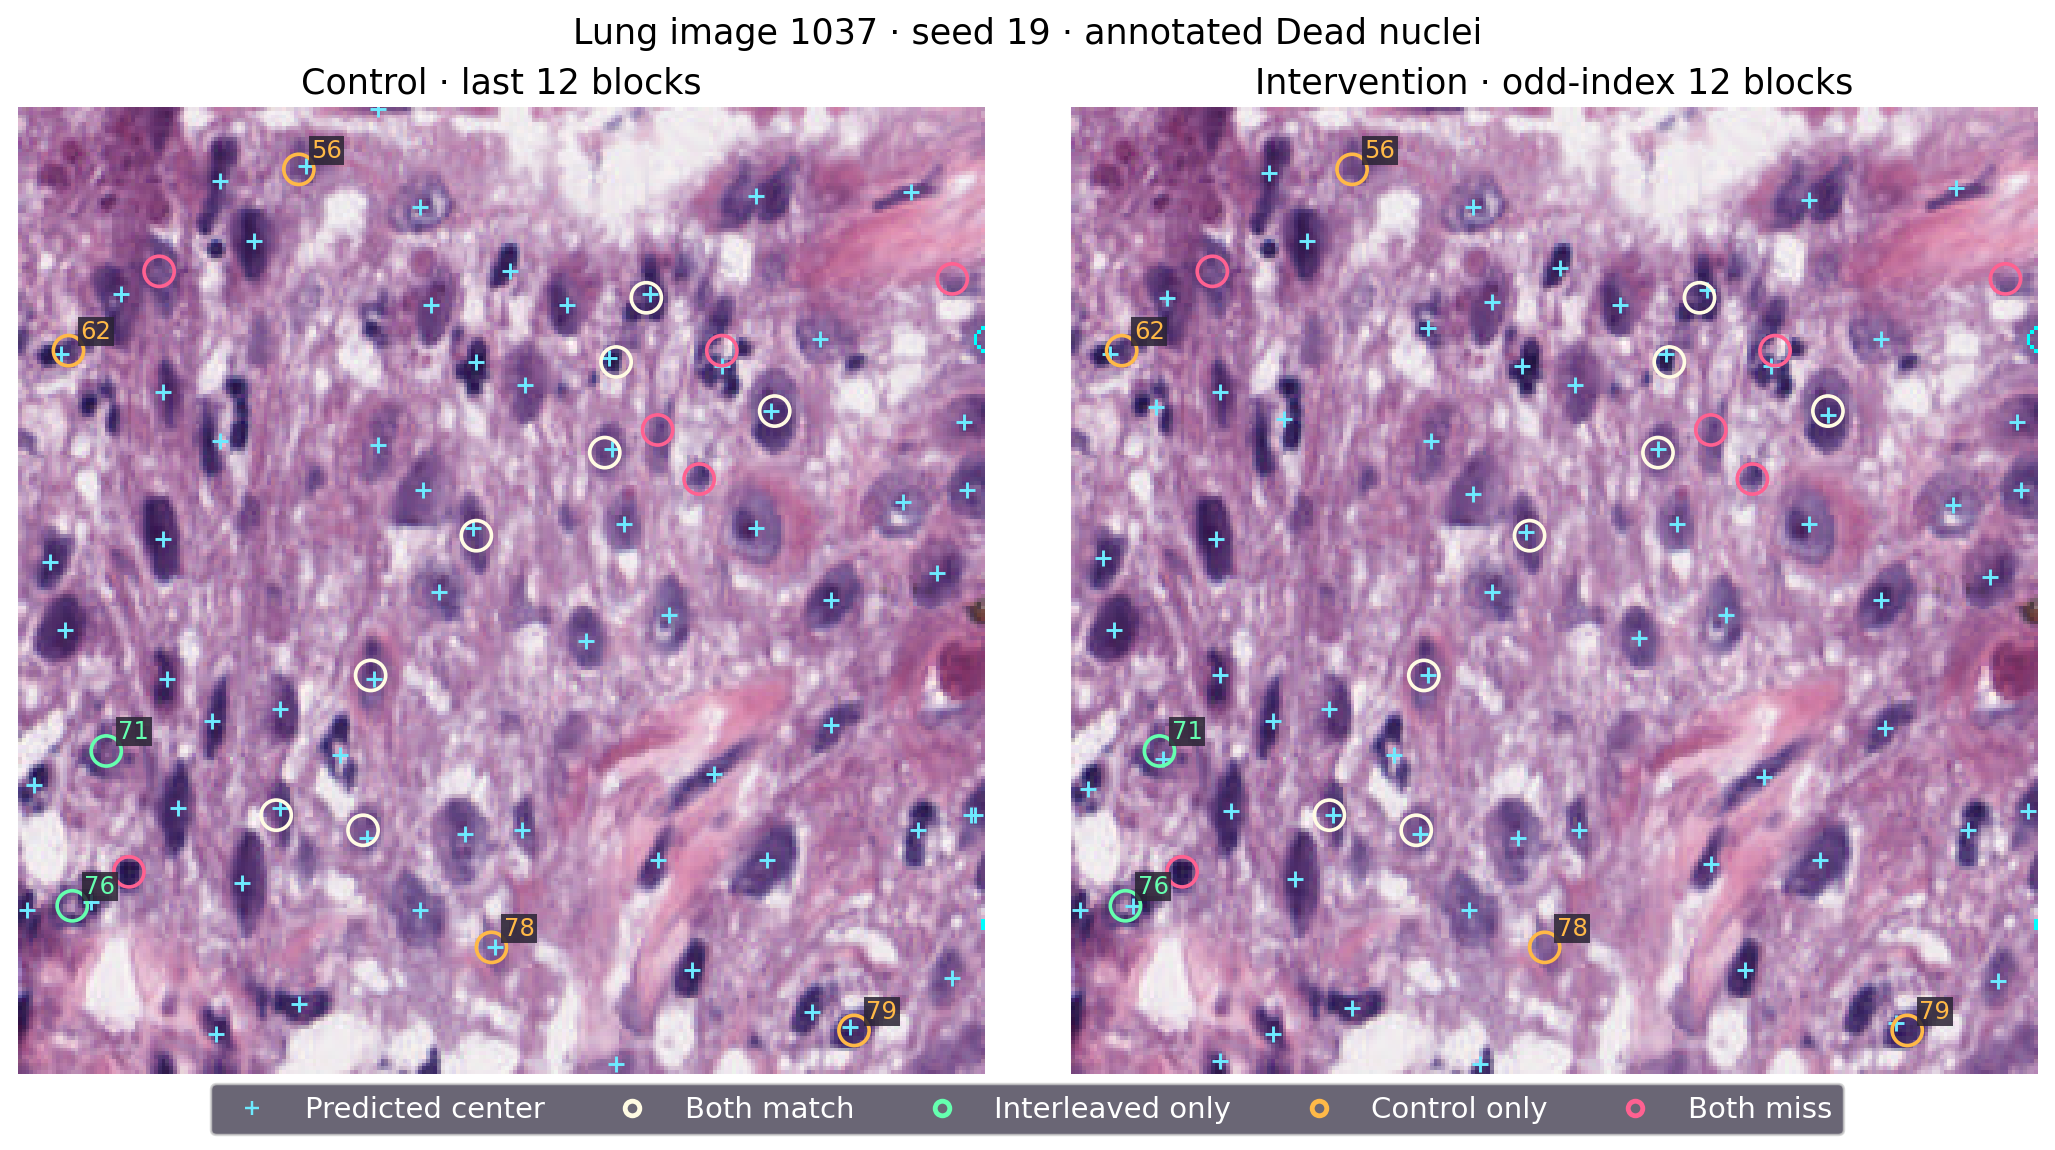
\includegraphics[width=\linewidth,height=.40\textheight,keepaspectratio]{assets/p28_image_1037_seed_19.png}
\captionof{figure}{P28 肺组织图像 1037，种子 19。左为后十二层对照，右为交错训练十二层；白、绿、橙、粉圆圈和青色十字的含义见上文。}
\raggedright

该图从 12/20 降至 10/20。对象 71 的最近预测距离从 21.02 降到 2.24 像素，变成匹配；对象 56 的距离从 2.24 增至 22.02，附近预测消失。对象 62 的距离从 2.24 移到 3.16，越过三像素匹配范围。这两种变化都影响计数。

\end{minipage}

\subsection{P29：前六层和后六层怎样改变结肠图像？}\label{p29ux524dux516dux5c42ux548cux540eux516dux5c42ux600eux6837ux6539ux53d8ux7ed3ux80a0ux56feux50cf}

\noindent

\begin{minipage}{\linewidth}\centering
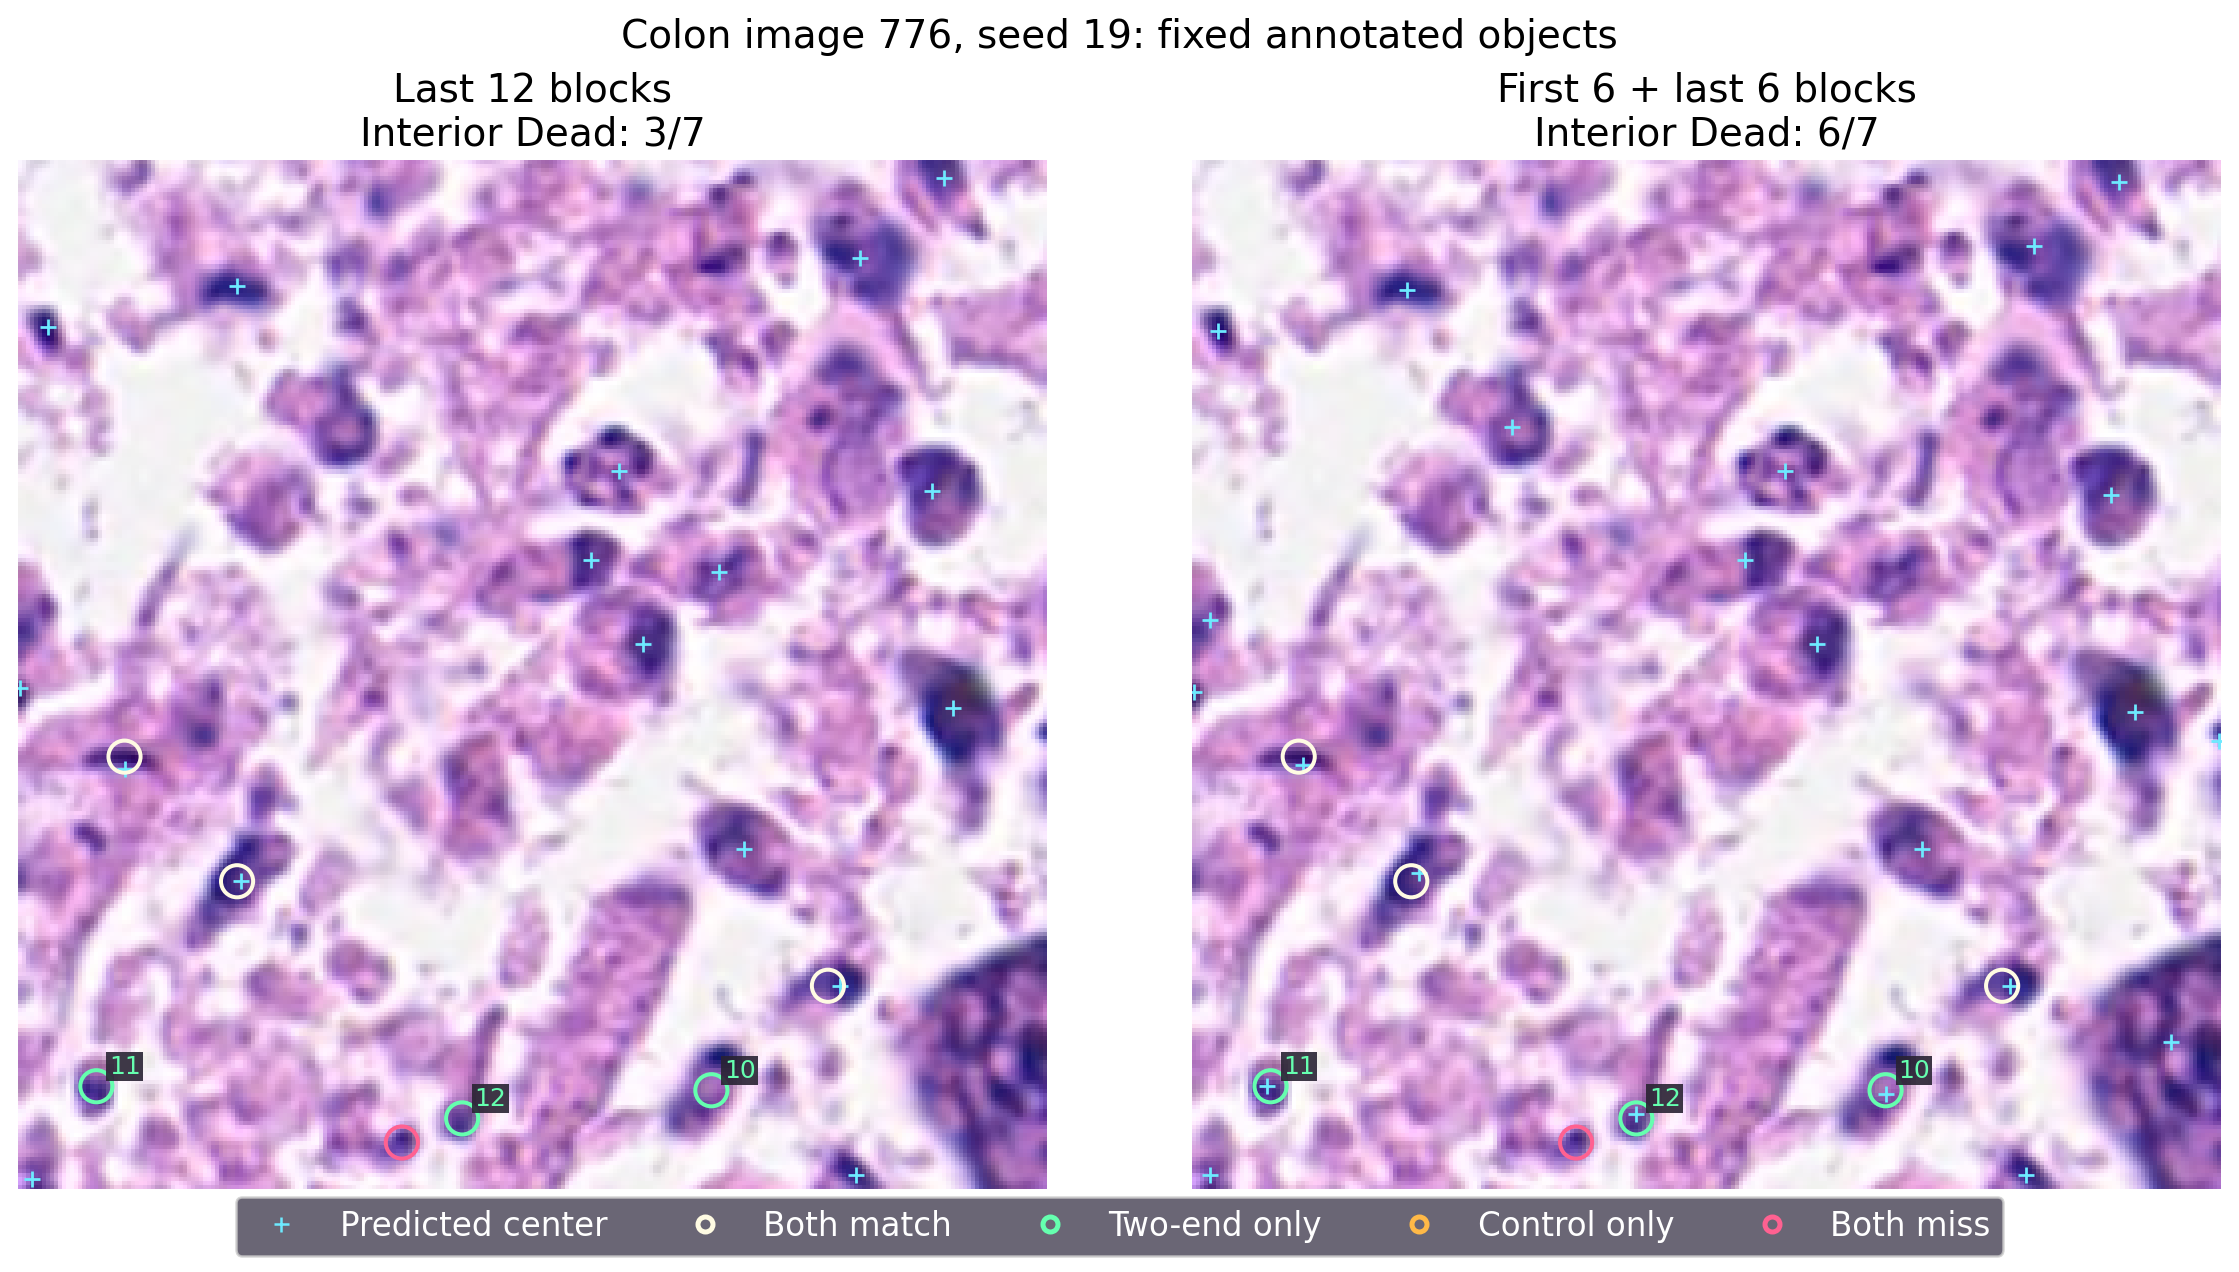
\includegraphics[width=\linewidth,height=.40\textheight,keepaspectratio]{assets/p29_image_776_seed_19.png}
\captionof{figure}{P29 结肠组织图像 776，种子 19。左为后十二层对照，右为前六层加后六层；标记含义见上文。}
\raggedright

该图从 3/7 增至 6/7。图像下方组织带的对象 10、11、12 在对照中附近缺少预测，新方案中最近点均距各自标注中心一像素。对象 12 位于（238，110），种子 1 也找到了它，最近预测距离从 61.52 降至 2 像素。两次训练都在同一标注位置出现了新增匹配。

\end{minipage}

\subsection{P30：找到更多核时，是否每张图都改善？}\label{p30ux627eux5230ux66f4ux591aux6838ux65f6ux662fux5426ux6bcfux5f20ux56feux90fdux6539ux5584}

\noindent

\begin{minipage}{\linewidth}\centering
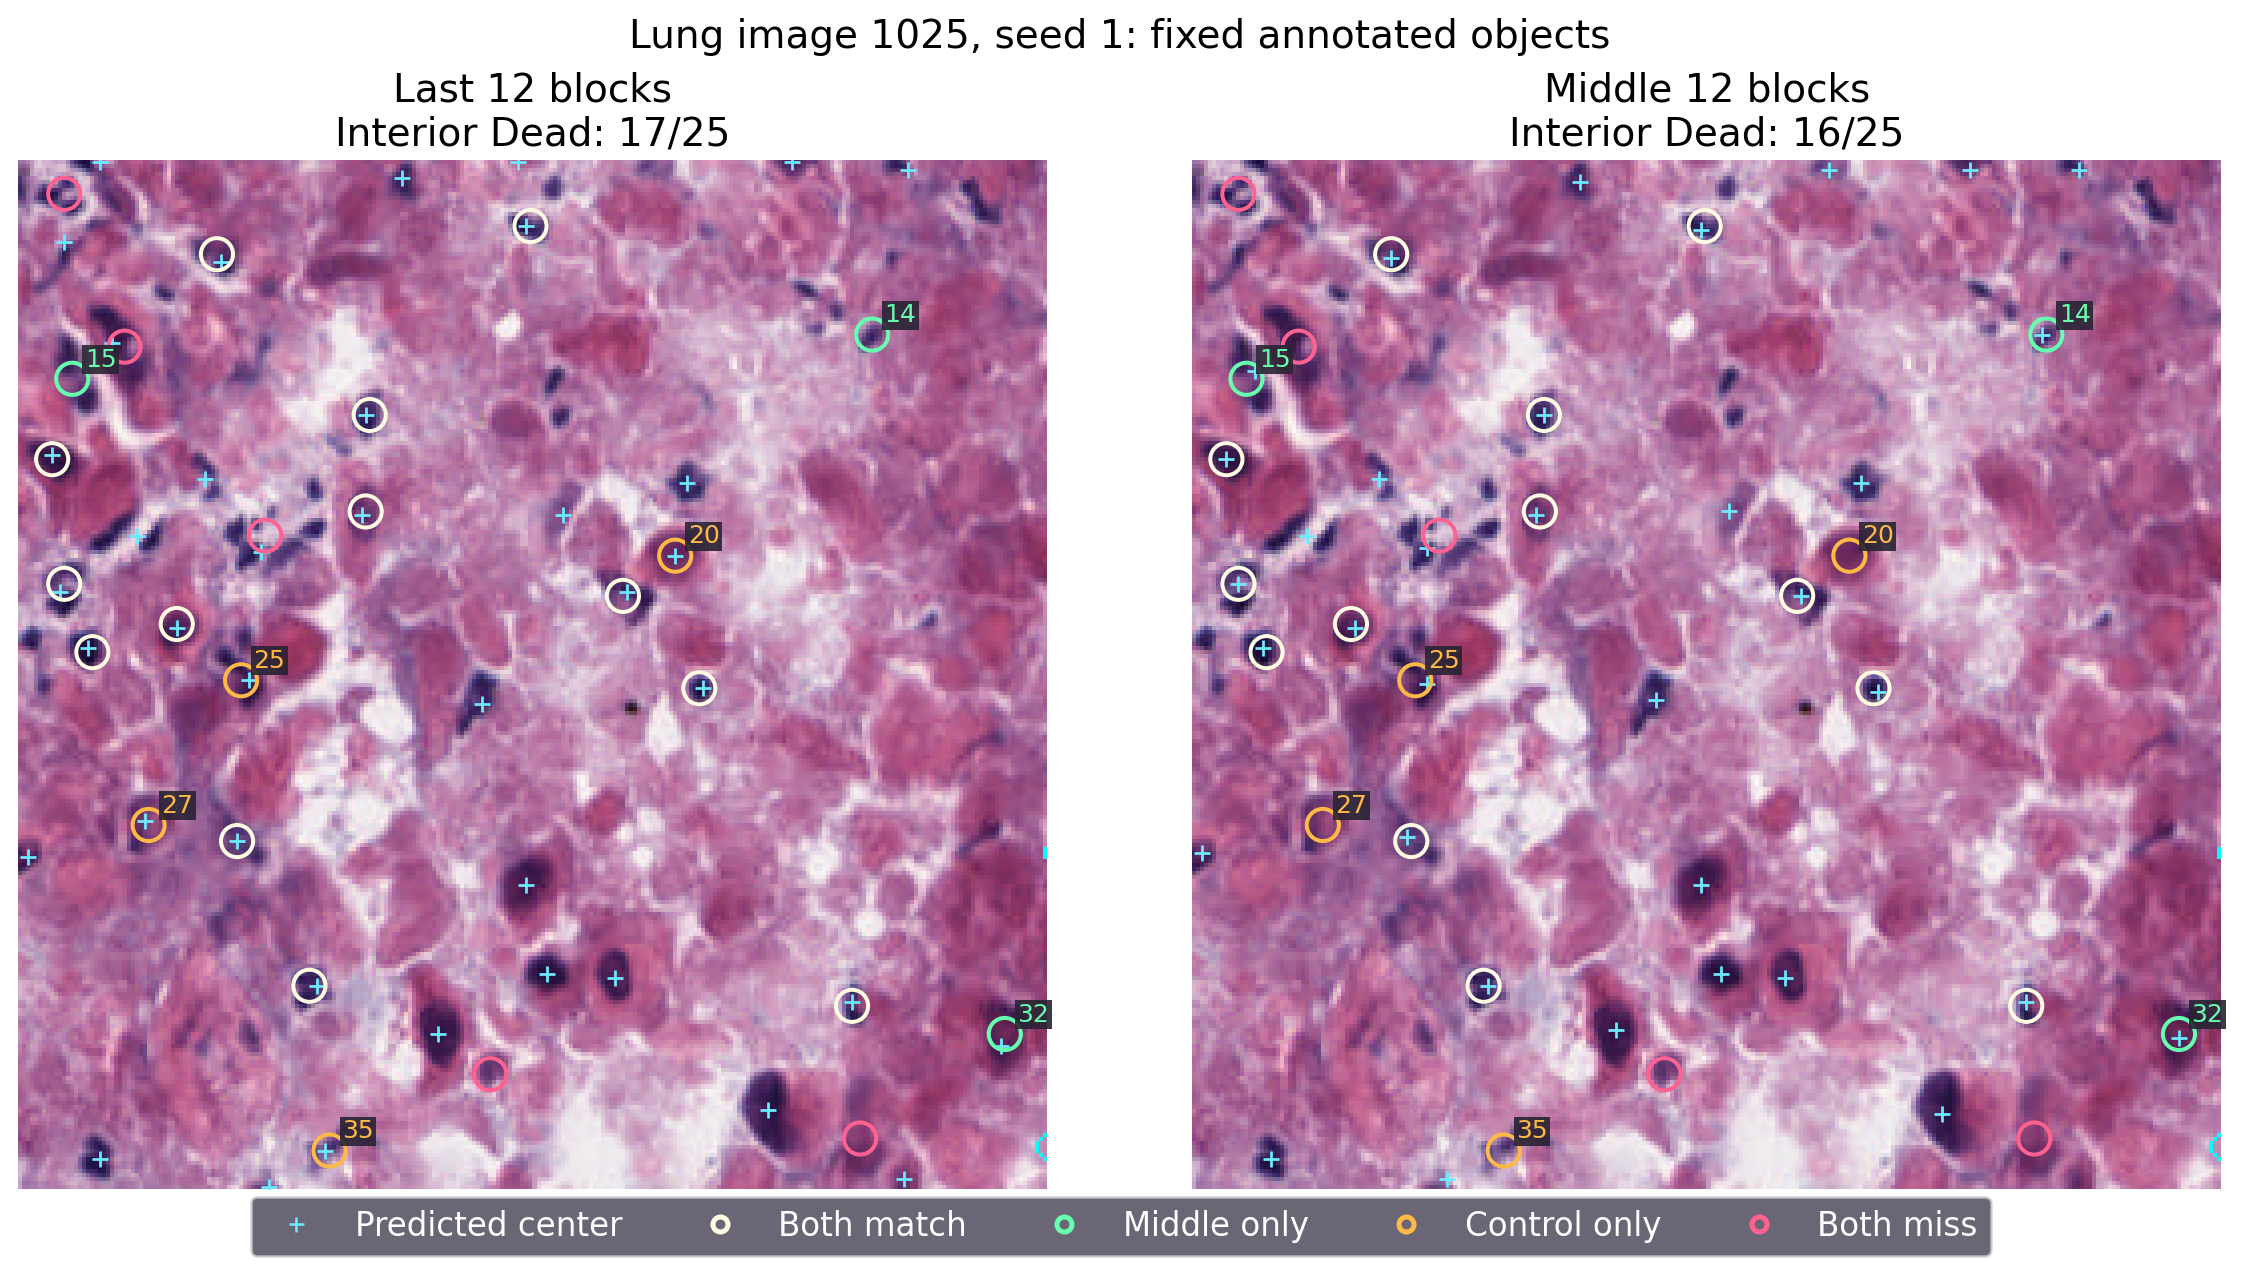
\includegraphics[width=\linewidth,height=.40\textheight,keepaspectratio]{assets/p30_image_1025_seed_1.png}
\captionof{figure}{P30 肺组织图像 1025，种子 1。左为后十二层对照，右为中间十二层；标记含义见上文。}
\raggedright

这张图从 17/25 降至 16/25：新增三个，同时丢失四个。面积为 31 平方像素的对象 14 从最近预测距离 41.98 降至 1 像素；对象 27 和 35 原先有匹配，新方案中附近预测距离分别增至 21.21 和 15.65 像素。两个种子的全部评估图像中，中间十二层方案分别多匹配 648 和 516 个细胞核。

\end{minipage}

\subsection{P31：改变检测头之后发生了什么？}\label{p31ux6539ux53d8ux68c0ux6d4bux5934ux4e4bux540eux53d1ux751fux4e86ux4ec0ux4e48}

\noindent

\begin{minipage}{\linewidth}\centering
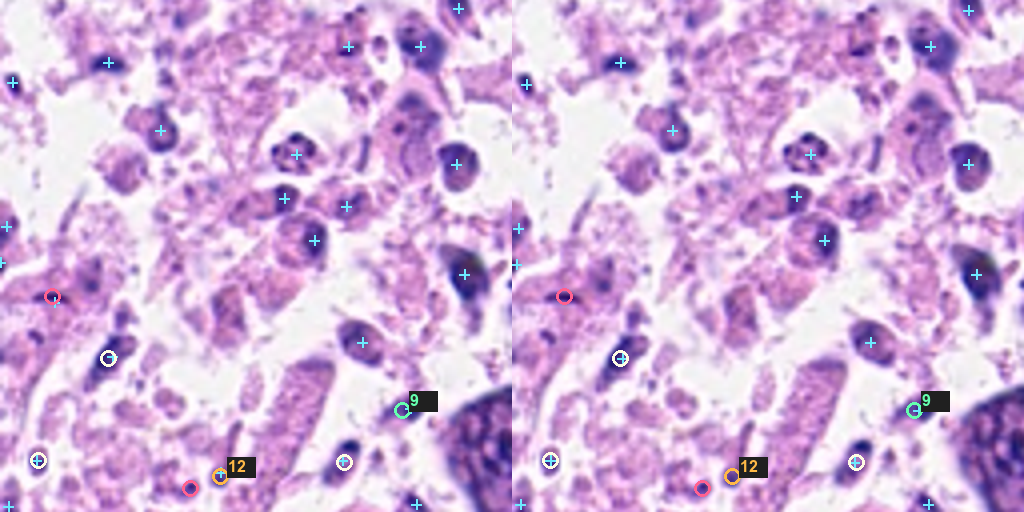
\includegraphics[width=\linewidth,height=.40\textheight,keepaspectratio]{assets/p31_image_776_seed_19.png}
\captionof{figure}{P31 结肠组织图像 776，种子 19。左为原检测头，右为加入分组归一化的检测头；标记含义见上文。}
\raggedright

该图两组都找到 7 个死亡核中的 4 个，但对象发生交换：对象 9 从距离 4.12 像素变成 2 像素，进入匹配范围；对象 12 从 2 像素变成 61.40 像素，附近预测消失。种子 1 的同一张图从 4/7 增至 6/7，两个对象均新增匹配。五轮结果和逐核坐标详见中英文报告与随附证据。

\end{minipage}

\end{document}
